\section{Results}
In this section, we discuss the evaluation results of \modelname, including pre-training performance and post-training outcomes. 
In addition, we provide comprehensive ablation studies that exam the model architecture and further discuss the observations of training \modelname.

\subsection{Pre-Training Training Loss Curve}
Figure~\ref{fig:135b_loss} shows the training loss curve of \modelname~during the entire pre-training. 
Each segment in the loss curve corresponds to one training stage, as described in Section~\ref{sec:hyper_params}. The loss curves demonstrate consistent descending trends across all training stages. For the second interval, although the descent rate moderated due to a constant learning rate, the performance metrics continued to show steady improvement throughout this interval.
\begin{figure}[htbp]
    \centering
    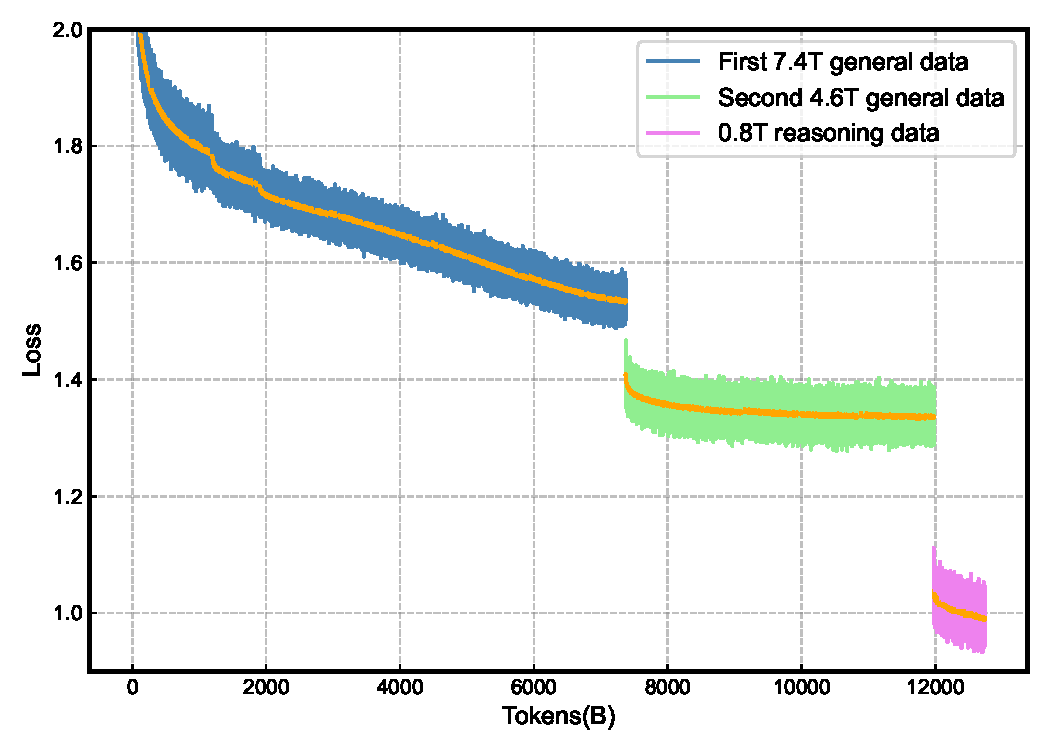
\includegraphics[width=0.7\textwidth]{fig/135B_loss.pdf}
    \caption{The training loss curve of \modelname~during the pre-training stage.}
    \label{fig:135b_loss}
\end{figure}

\paragraph{Zero loss spike} As shown in Figure~\ref{fig:135b_loss}, \textbf{no loss spikes} occur throughout the entire pre-training process.
While such spikes are common in LLM training \cite{takase2024spikemore}, the absence of them here underscores the importance of our depth-scaled sandwich norm and TinyInit in ensuring stable training.
The negative effect of loss spike to the model performance will be further elaborated in Section~\ref{sec:sandwich-ablation}.



\subsection{Pre-Training Stage}
\paragraph{Benchmarks} We evaluate \modelname{} base model across multiple domains using open-source benchmarks, including language understanding, question answering, code generation, and math problem solving. The evaluation mainly uses English and Chinese test sets, with some additional multilingual benchmarks for broader coverage.

\begin{itemize}[leftmargin=*]

\item Language understanding: We employ \textit{Hellaswag} \cite{Zellers2019HellaSwagCA} and \textit{Winogrande} for contextual reasoning tasks, \textit{DROP} \cite{Dua2019DROPAR}, \textit{RACE} \cite{Lai2017RACELR}, and \textit{ARC} \cite{Clark2018ThinkYH} series for comprehensive reading comprehension evaluation, along with \textit{PIQA} \cite{Bisk2019PIQARA}, \textit{Natural Questions} \cite{Kwiatkowski2019NaturalQA} and \textit{TriviaQA} \cite{Joshi2017TriviaQAAL} to assess knowledge retrieval.

\item Question answering: The assessment includes \textit{C-Eval} \cite{Huang2023CEvalAM} for Chinese knowledge, \textit{MMLU} \cite{Hendrycks2020MeasuringMM} and its advanced variant \textit{MMLU-Pro} \cite{Wang2024MMLUProAM} for English domain knowledge, supplemented by \textit{BigBenchHard} \cite{Suzgun2022ChallengingBT} to evaluate creative problem-solving

\item Code generation and understanding: We utilize \textit{HumanEval} \cite{Chen2021EvaluatingLL} and \textit{MBPP} \cite{Austin2021ProgramSW} for standard code generation tasks, while \textit{CruxEval} \cite{Gu2024CRUXEvalAB} for code understanding and reasoning.

\item Mathematical Reasoning : We measure skills with \textit{CMath} \cite{Wei2023CMATHCY} and \textit{GSM8K} \cite{Cobbe2021TrainingVT} for fundamental arithmetic and simple problems, \textit{MATH} \cite{Hendrycks2021MeasuringMP} for advanced mathematical reasoning, and \textit{MGSM} \cite{Shi2022LanguageMA} for multilingual math problem solving.

\end{itemize}

\paragraph{Baselines \& Comparison Settings} We compare \modelname~against several strong baselines covers both dense models (Qwen2.5-72B, Llama-405B) and MoE architectures (DeepSeek-V3). For base models, the majority of our evaluations employ few-shot inputs, with a minority using zero-shot prompts. We evaluate most benchmarks with gold answers through exact matching, while employing execution-based verification for code generation tasks.

\paragraph{Evaluation Results}
In Table~\ref{tab:main}, we compare the pre-trained base model of \modelname~with other leading models. Overall, \modelname~achieves state-of-the-art performance on most general English benchmarks and all Chinese benchmarks.
While it trails DeepSeek V3 on code and math-related tasks, it performs competitively on these domains.

A closer examination reveals that \modelname~excels on Chinese benchmarks, surpassing both Qwen 2.5 72B and DeepSeek V3, the current best-performing Chinese model. 
In addition, when compared to Llama 3.1 405B, \modelname~achieves better scores on most of the challenging benchmarks, while utilizing only about 29\% of the training FLOPs required by Llama 405B.
These results suggest the effectiveness of our model architecture and the high quality of our training data.


\begin{table}[!h]
    \centering
    \footnotesize
    \setlength{\tabcolsep}{4.5pt}
    \caption{Comparison of \modelname~and other representative models across a diverse set of benchmarks for evaluating language, coding and mathematical skills. Bold values represent the best results in each line, and underlined values represent \modelname~is the best among dense models.}
    \small
    \begin{tabular}{@{}c l c | c c c | c@{}}
    \toprule
    & \multirow{2}{*}{\centering \textbf{Benchmark {\tiny (Metric)}}} & \multirow{2}{*}{\textbf{\# Shots}} & \textbf{Qwen2.5} & \textbf{Llama-3.1} & \textbf{DeepSeek} & \textbf{\modelname} \\
    & & & \textbf{72B Base} & \textbf{405B Base} & \textbf{V3 Base} & \textbf{Base} \\
    \midrule
    & Architecture & - & Dense & Dense & MoE & Dense \\
    & \# Activated Params & - & 72B & 405B & 37B & 135B \\
    & \# Total Params & - & 72B & 405B & 671B & 135B \\
    \midrule
    \multirow{16}{*}{English} & BBH {\tiny (EM)} & 3-shot & 79.8 & 82.9 & \textbf{87.5} & 79.1 \\
    & MMLU {\tiny (EM)} & 5-shot & 85.0 & 84.4 & \textbf{87.1} & \underline{85.4}  \\
    & MMLU-Pro {\tiny (EM)} & 5-shot & 58.3 & 52.8 & \textbf{64.4} & \underline{63.1}  \\
    & DROP {\tiny (F1)} & 3-shot & 80.6 & 86.0 & \textbf{89.0} & 61.0  \\
    & ARC-Easy {\tiny (EM)} & 25-shot & 98.4 & 98.4 & 98.9 & \textbf{100.0} \\
    & ARC-Challenge {\tiny (EM)} & 25-shot & 94.5 & 95.3 & 95.3 & \textbf{97.0}  \\
    & HellaSwag {\tiny (EM)} & 10-shot & 84.8 & 89.2 & 88.9 & \textbf{99.0}  \\
    & PIQA {\tiny (EM)} & 0-shot & 82.6 & 85.9 & 84.7 & \textbf{98.0} \\
    & WinoGrande {\tiny (EM)} & 5-shot & 82.3 & 85.2 & 84.9 & \textbf{91.0}  \\
    & RACE-Middle {\tiny (EM)} & 5-shot & 68.1 & 74.2 & 67.1 & \textbf{97.0} \\
    & RACE-High {\tiny (EM)} & 5-shot & 50.3 & 56.8 & 51.3 & \textbf{97.0} \\
    & TriviaQA {\tiny (EM)} & 5-shot& 71.9 & 82.7 & 82.9 & \textbf{90.5} \\
    & NaturalQuestions {\tiny (EM)} & 5-shot & 33.2 & 41.5 & 40.0 & \textbf{52.7} \\
    & AGIEval {\tiny (EM)} & 0-shot & 75.8 & 60.6 & 79.6 & \textbf{80.4} \\
    \midrule
    \multirow{4}{*}{Code} & HumanEval {\tiny (Pass@1)} & 0-shot & 53.0 & 54.9 & 65.2 & \textbf{81.1} \\
    & MBPP {\tiny (Pass@1)} & 3-shot & 72.6 & 68.4 & \textbf{75.4} & 72  \\
    & CRUXEval-I {\tiny (EM)} & 2-shot & 59.1 & 58.5 & \textbf{67.3} & \underline{61.8}  \\
    & CRUXEval-O {\tiny (EM)} & 2-shot & 59.9 & 59.9 & \textbf{69.8} & \underline{61.5}  \\
    \midrule
    \multirow{3}{*}{Math} 
    & GSM8K {\tiny (EM)} & 8-shot & 88.3 & 83.5 & \textbf{89.3} & \textbf{89.3}  \\
    & MATH {\tiny (EM)} & 4-shot & 54.4 & 49.0 & 61.6 & \textbf{62.5}  \\
    & MGSM {\tiny (EM)} & 8-shot & 76.2 & 69.9 & \textbf{79.8} & 75.1  \\
    & CMath {\tiny (EM)} & 3-shot & 84.5 & 77.3 & \textbf{90.7} & 78.2  \\
    \midrule
    \multirow{7}{*}{Chinese} & CLUEWSC {\tiny (EM)} & 5-shot & 82.5 & 83.0 & 82.7 & \textbf{95.0} \\
    & C-Eval {\tiny (EM)} & 5-shot & 89.2 & 72.5 & 90.1 & \textbf{90.3}  \\
    & CMMLU {\tiny (EM)} & 5-shot & 89.5 & 73.7 & 88.8 & \textbf{91.7} \\
    & CMRC {\tiny (EM)} & 1-shot & 75.8 & 76.0 & 76.3 & \textbf{86.0}  \\
    & C3 {\tiny (EM)} & 0-shot & 76.7 & 79.7 & 78.6 & \textbf{99.0} \\
    & CCPM {\tiny (EM)} & 0-shot & 88.5 & 78.6 & 92.0 & \textbf{93.0}  \\
    \bottomrule
    \end{tabular}
    \label{tab:main}
\end{table}


\subsection{Post-Training and Reasoning Capability}
\paragraph{Benchmarks} We conduct a comprehensive evaluation of the \modelname's capabilities over reasoning and non-reasoning tasks:

\begin{itemize}[leftmargin=*]
\item Sophisticated reasoning tasks encompass three specialized subcategories: mathematical competence measured by \textit{AIME 2024}~\cite{MAA} and \textit{MATH-500}, Coding competition benchmarks \textit{LiveCodeBench}~\cite{jain2024livecodebench} and scientific reasoning task \textit{GPQA Diamond}~\cite{rein2024gpqa};
\item General language comprehension and reasoning capabilities, represented by \textit{MMLU-Pro}~\cite{gema2024we}, \textit{Arena Hard}~\cite{arenahard2024}.
\end{itemize}


\paragraph{Baselines \& Comparison Settings} We compare \modelname~against strong baselines including GPT-4o-0513, reasoning models DeepSeek-R1, Hunyuan-T1 and large dense models, Qwen2.5-72B-Instruct and Mistral-Large 2. 
We use Pass@1  averaged over multiple independent runs as the evaluation metric to assess the performance.

\paragraph{Evaluation Results}
In Table~\ref{tab:StandardBenchmarks}, we compare the evaluation results of \modelname~with other baseline models. \modelname~achieves state-of-the-art performance on the reasoning benchmarks including AIME 2024, MATH-500, GPQA and LiveCodeBench, while maintaining strong capabilities in general language comprehension tasks.

When compared to dense LLMs (Qwen and Mistral-Large 2), \modelname~shows particularly significant advantages in reasoning tasks. This superior performance stems from the 0.8T reasoning-focused data used in pre-training (Section~\ref{sec:hyper_params}). The reasoning-enhanced base model substantially benefits subsequent post-training phases.



\begin{table}[!h]
    \centering
    \caption{Comparison of \modelname~models and other representative models across benchmarks. $\dagger$ indicates results from Artificial Analysis \cite{ai_analysis}.}
    \resizebox{\linewidth}{!}{
    \small
    \begin{tabular}{@{}l *{6}{c} @{}}
    
    \toprule
    \multirow{2}{*}{\centering\textbf{Model}} & \multirow{2}{*}{\textbf{AIME 2024}} & \multirow{2}{*}{\textbf{MATH-500}} & \textbf{GPQA} & \textbf{LiveCode} & \multirow{2}{*}{\textbf{ArenaHard}}& \multirow{2}{*}{\textbf{MMLU-pro}} \\
    &  &  & \textbf{Diamond} & \textbf{Bench} &  \\
     \midrule
    \textbf{GPT-4o-0513} & 9.3 & 74.6 & 49.9 & 32.9 & 80.4 & 72.6 \\
    \textbf{Qwen2.5-72B} & 16.0 & 83.1 & 49 & 27.6 & 81.2 & 72.0 \\
    \textbf{Mistral-Large 2}$^\dagger$ & 11.0 & 73.6 & 48.6 & 29.3 & - & 69.7 \\
    \textbf{Hunyuan-T1} & 79.8 & 96.2 & 69.3 & 64.9 & 91.9 & \textbf{87.2} \\
    \textbf{DeepSeek-R1} & 79.8 & 97.3 & 71.5 &  65.9 & \textbf{92.3} &  84.0\\
    \midrule
    \textbf{\modelname} & \textbf{80.8} & \textbf{97.4} & \textbf{74.2} & \textbf{66.5} & 91.5 & 84.4 \\
    \bottomrule
    \end{tabular}
    }
    \label{tab:StandardBenchmarks}
\end{table}

\subsection{Ablation Studies}  
This section presents additional ablation studies of the model architecture and analyzes key training behaviors to facilitate a deeper understanding and discussion of dense LLM training.

\subsubsection{Depth-scaled Sandwich-norm} \label{sec:sandwich-ablation}
We conducted experiments to validate the effectiveness of depth-scaled sandwich norm compared to pre-norm architectures. Using a dense Transformer model with 13 billion parameters trained on 300 billion tokens with identical hyperparameters for both configurations, we observe significant improvements.

Figure~\ref{fig:sandwich_compare} shows the depth-scaled sandwich-norm architecture stabilizes gradient norms and effectively eliminates loss spikes, leading to faster training convergence.
We evaluated performance on two composite benchmarks: EN basic, consisting of multiple English benchmarks, and ZH basic, representing Chinese benchmarks. Additional evaluation using LAMBADA \cite{Paperno2016TheLD} (English) and WPLC \cite{Ge2021ChineseWA} (Chinese) next-token prediction tasks confirmed the advantage of applying depth-scaled sandwich-norm. 
The results clearly suggest that preventing loss spikes during pre-training is crucial for optimal model performance.


\begin{figure}[htbp]
  \centering
  \subfloat[Loss]{
    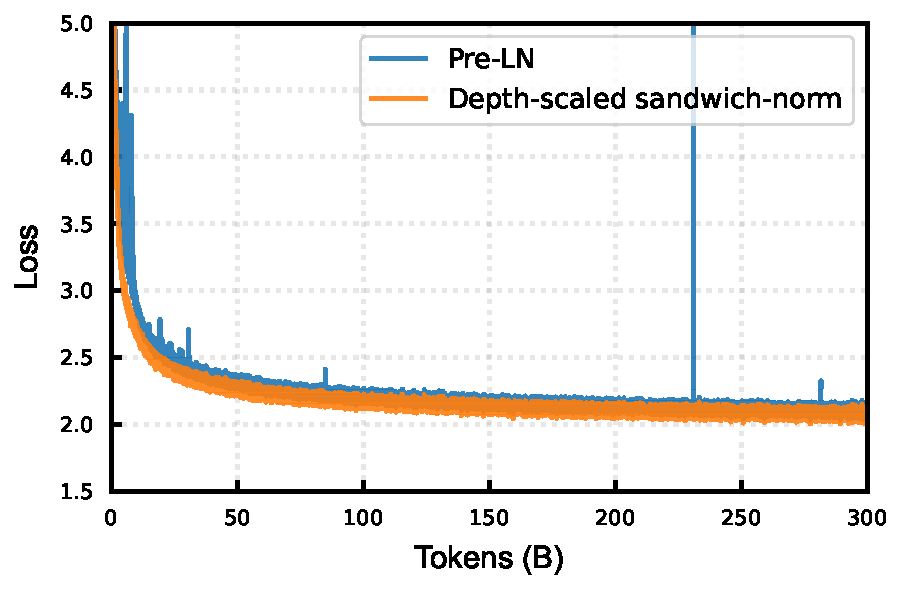
\includegraphics[width=0.47\textwidth]{fig/sandwichnorm-loss.pdf}
    % \label{fig:sub1}
  }
  \hfill
  \subfloat[Gradient norm]{
    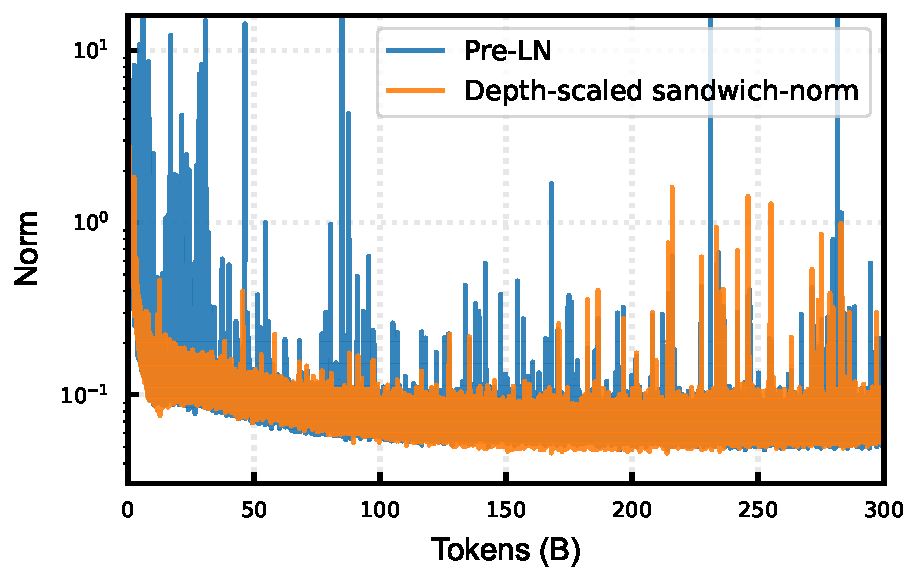
\includegraphics[width=0.48\textwidth]{fig/sandwich_norm.pdf}
    % \label{fig:sub2}
  }
  \caption{Pre-training loss and gradient norm for a 13B model using Pre-LN and Depth-Scaled Sandwich-Norm (DSSN). The curves with Pre-LN has significant spikes, which harm the trained model, while the curves of DSSN are much smoother.  }
  \label{fig:sandwich_compare}
\end{figure}


\begin{table}[h]
	\centering
    \small
	\caption{Performance comparison between Pre-LN and Depth-scaled Sandwich-Norm.}
    \label{tab:sandwich_compare}
	\setlength{\tabcolsep}{8.0pt}
	\begin{tabular}{cccccc}
		\toprule
		\textbf{Model} & \textbf{Tokens (B)} & \textbf{EN basic} & \textbf{ZH basic} & \textbf{LAMBADA} & \textbf{WPLC} \\
		\midrule
		Pre-LN & 300 & 0.42 & 0.52 & 0.675 & 0.194 \\
		Depth-scaled sandwich-norm & 300 & 0.45 & 0.54 & 0.693 & 0.224 \\
		\bottomrule
	\end{tabular}
\end{table}

To further ablate the effect of our depth-scaled factor in RMSNorm initialization, we compare with the plain sandwich-norm that does not have the $\sqrt{L}$ scaling factor in Eq.~\eqref{eq:sandwich}. 
Here, we use a proxy model containing 1.6 billion parameters and 94 layers, which has the same depth with \modelname. 
By using this proxy model, we examine the effectiveness of sandwich-norm on training very deep Transformers. 
In Figure~\ref{fig:1.6B_94l}, we can observe some loss spikes with the plain sandwich-norm, but our depth-scaled sandwich-norm can be trained smoothly, and attains lower loss.

\begin{figure}[htbp]
    \centering
    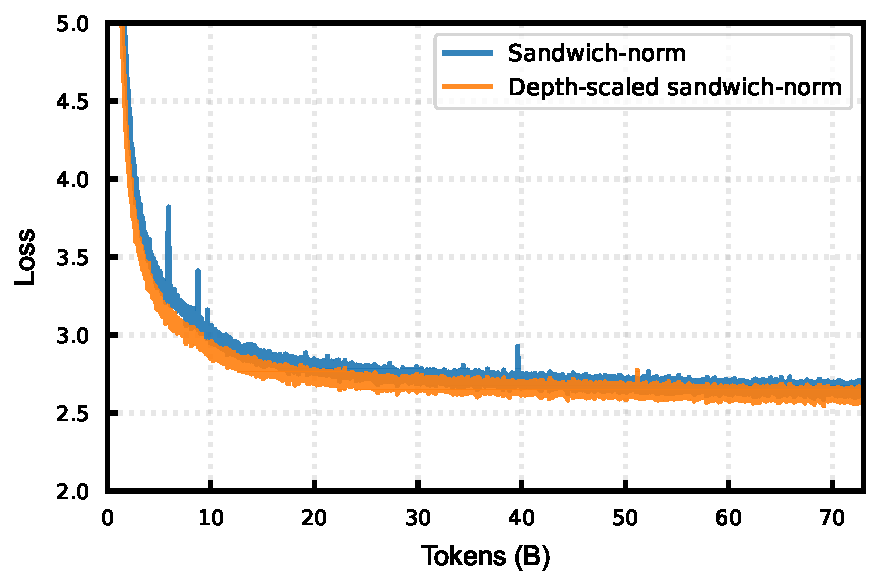
\includegraphics[width=0.6\textwidth]{fig/1.6B_94l.pdf}
    \caption{Pre-training loss for a 94-layer 1.6B model using original and depth-scaled sandwich-norm. The original sandwich-norm still suffers loss spikes during training.}
    \label{fig:1.6B_94l}
\end{figure}

\subsubsection{Tiny Initialization}
We conduct experiments to study the effectiveness of TinyInit proposed in Section~\ref{sec:tinyinit}.
After being trained on 102 billion tokens, \modelname{} initialized with TinyInit strategy, with standard deviation $\sqrt{\frac{1}{2dL}}$), performs significantly better than the baseline model that utilizes traditional initialization, whose standard deviations are $\sqrt{\frac{2}{5d}}$ and $\sqrt{\frac{2}{5dL}}$. The results are shown in Table~\ref{tab:tinyinit_exp}. BIG-bench (aug) is a test set developed internally through data augmentation of the original BIG-bench, designed to mitigate the impact of test set leakage.
\begin{table}[h]
	\centering
        \small
	\caption{Performance comparison of traditional initialization and TinyInit.} \label{tab:tinyinit_exp}
	% \setlength{\tabcolsep}{8.0pt}
	\begin{tabular}{ccccccccc}
		\toprule
		\textbf{Model} & \textbf{Tokens (B)} & \textbf{EN basic} & \textbf{ZH basic} & \textbf{LAMBADA} & \textbf{WPLC} & \textbf{C-Eval} & \textbf{MMLU} & \textbf{BIG-bench (aug)} \\
		\midrule
		Baseline & 102 & 0.444 & 0.538 & 0.694 & 0.229 & 0.476 & 0.473 & 0.357 \\
		TinyInit & 102 & 0.456 & 0.537 & 0.727 & 0.257 & 0.524 & 0.502 & 0.384 \\
		\bottomrule
	\end{tabular}
\end{table}

\subsubsection{Layer Statistics of \modelname}

\paragraph{Stable activation scale}
Figure~\ref{fig:act_analysis} presents the activation patterns of attention and FFN modules across Transformer layers, showing the mean, standard deviation, and top-1 activation values. The activation distributions demonstrate stability, with standard deviations maintaining consistent scales throughout pre-training while preserving a clear layer-wise pattern.
Our analysis reveals the presence of ``super activations'', whose magnitude reaches $10^3$ magnitude in shallow layers, a phenomenon consistent with findings in the Llama model~\cite{Yu2024TheSW}.
Notably, Figure~\ref{fig:act_analysis} illustrates that these top-1 activation values progressively decrease with layer depth, indicating that their influence becomes relatively small on the final output.

\begin{figure}[htbp]
    \centering
    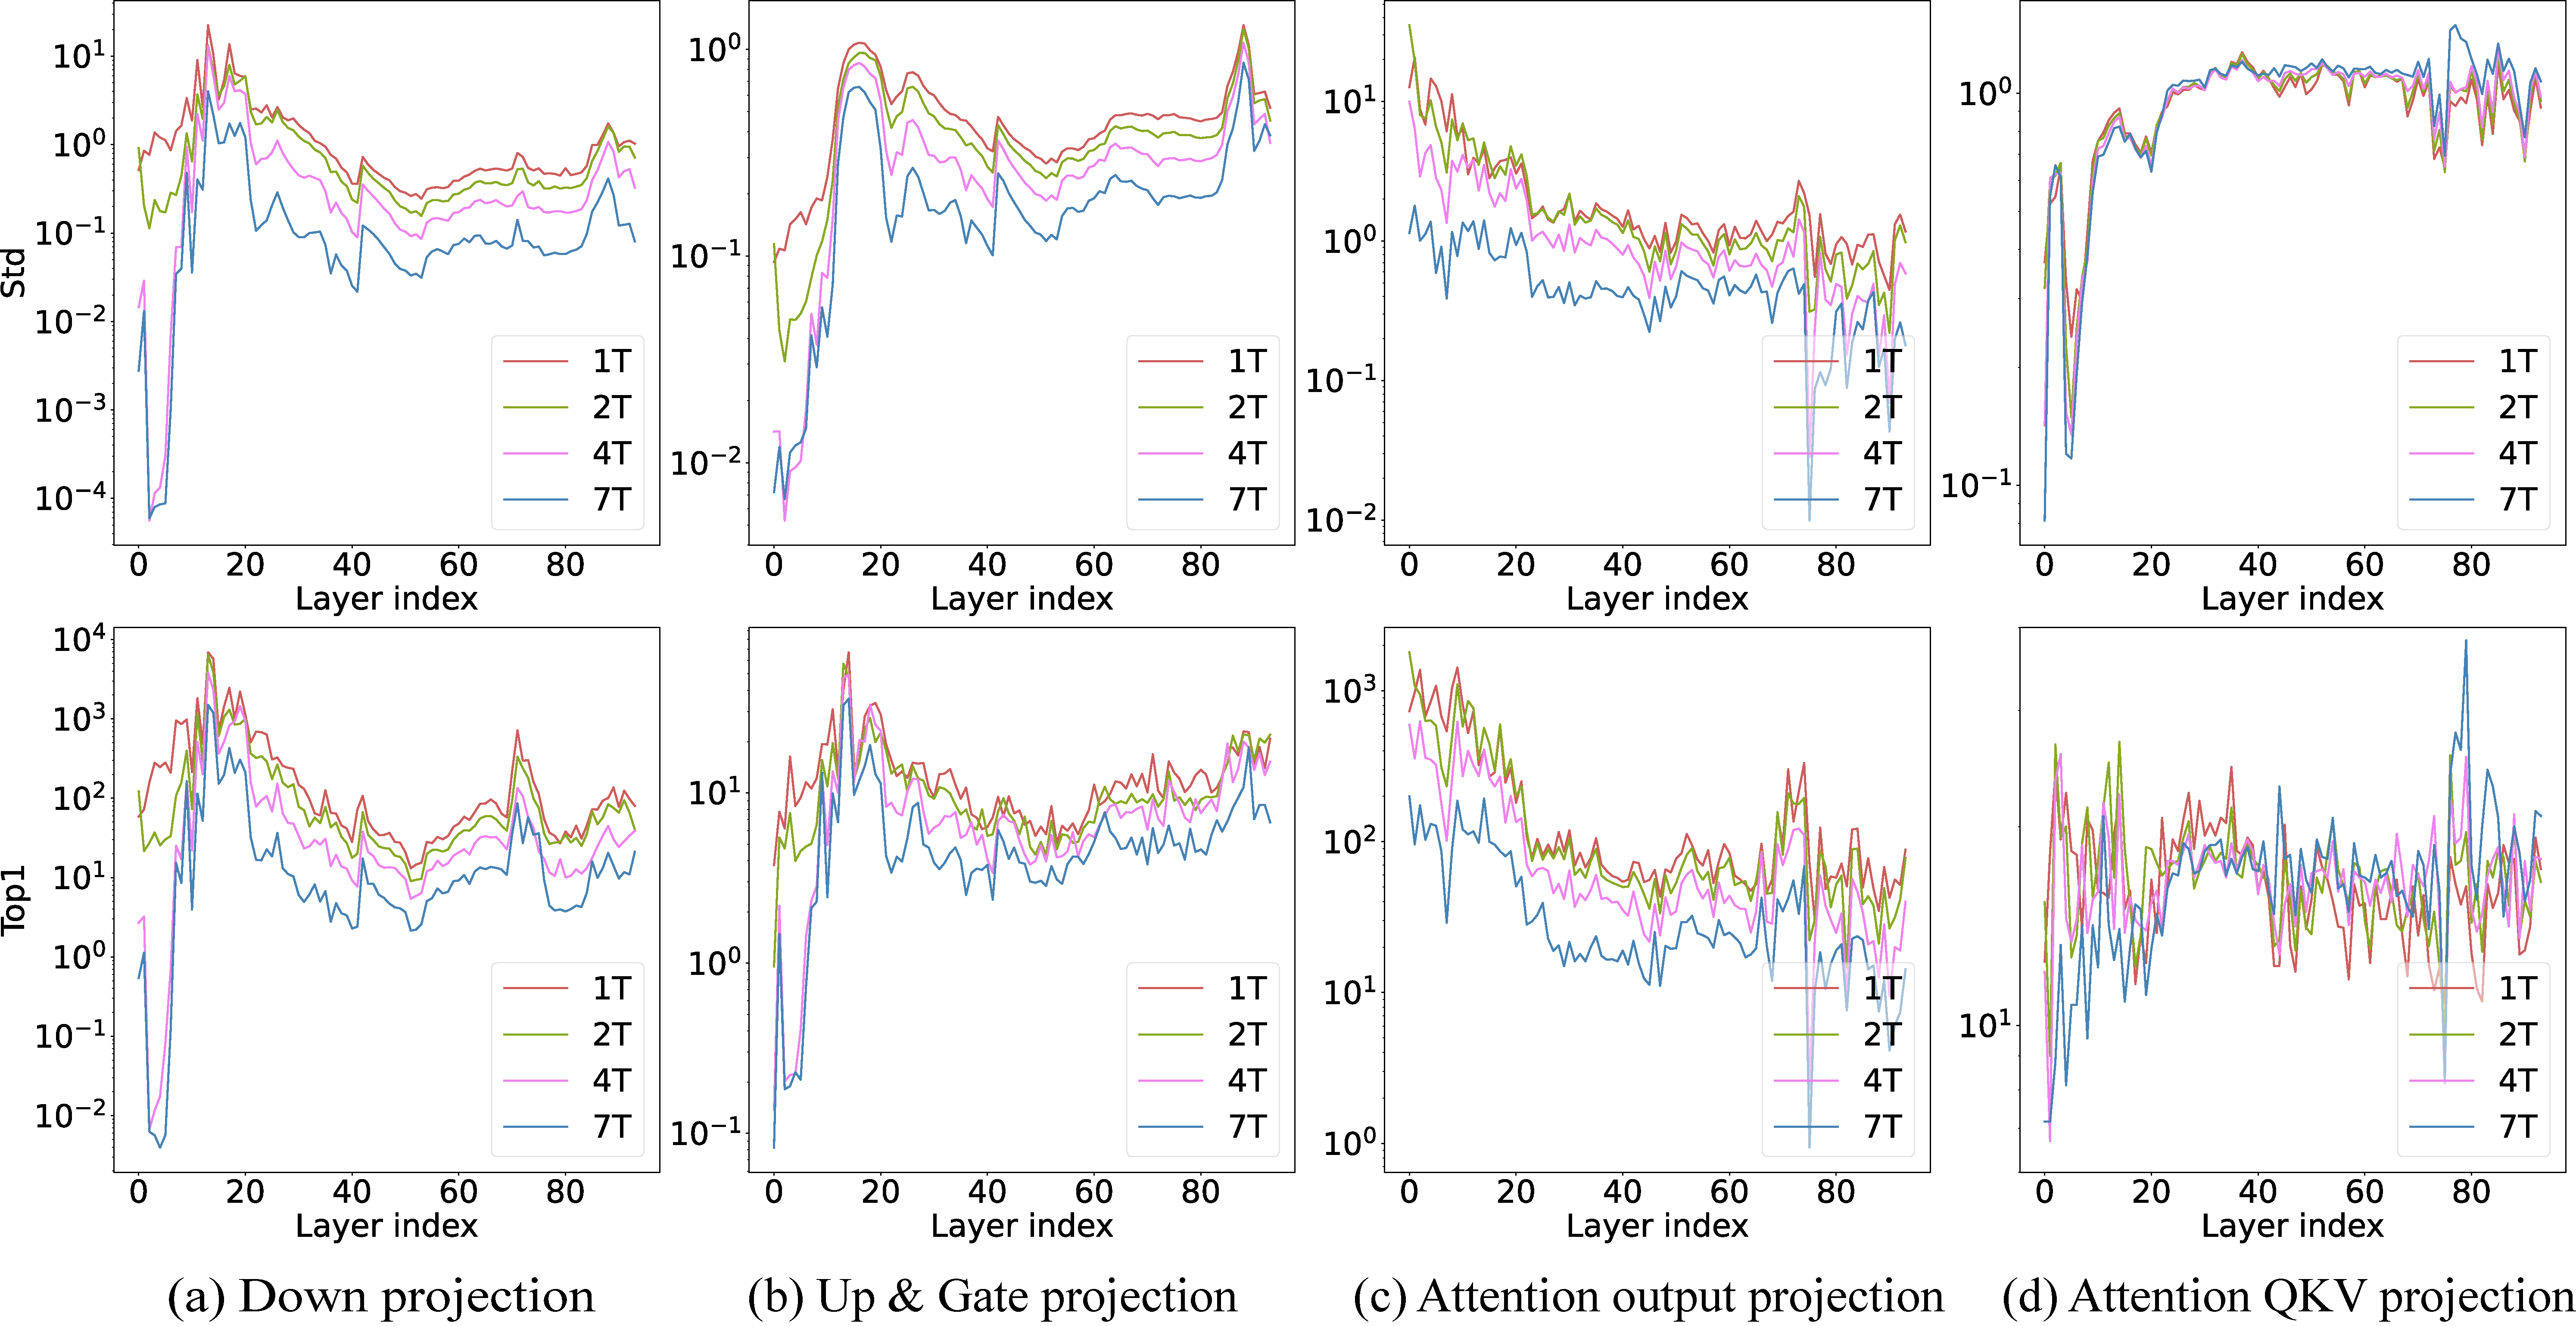
\includegraphics[width=\textwidth]{fig/model_iter_7T_activation.pdf}
    \caption{Activation of attention and FFN modules. Mean, standard deviation, and top-1 value of activations are included. Each line represents different training tokens from 1T, 2T, 4T to 7T. The "Std" row shows the stable activation scale across layers. The "Top 1" row shows the existence of the "super activations" in down projection and attention output projection, with magnitudes falling within a reasonable range and comparable to those observed in the LLaMA model~\cite{Yu2024TheSW}.}
    \label{fig:act_analysis}
\end{figure}



\paragraph{Layer-wise patterns of depth-scaled sandwich norm.}

Figure~\ref{fig:gamma_analysis} presents the distribution of scaling parameters $\gamma$ across all sandwich-norm layers, revealing several key observations:
All four LayerNorm $\gamma$ parameters exhibit decreasing mean/standard deviation during training, consistent with weight decay effects.
Post-norm $\gamma$ values show layer-dependent patterns:
The standard deviation of post-norm $\gamma$ increases substantially with layer depth.
Pre-norm $\gamma$ maintains relatively constant standard deviation across layers.
This pattern suggests an intriguing model behavior: shallow layers rely primarily on residual connections, while deeper layers progressively emphasize transformer layer outputs as the scaling factor $\gamma$ grows in magnitude.
\begin{figure}[htbp]
    \centering
    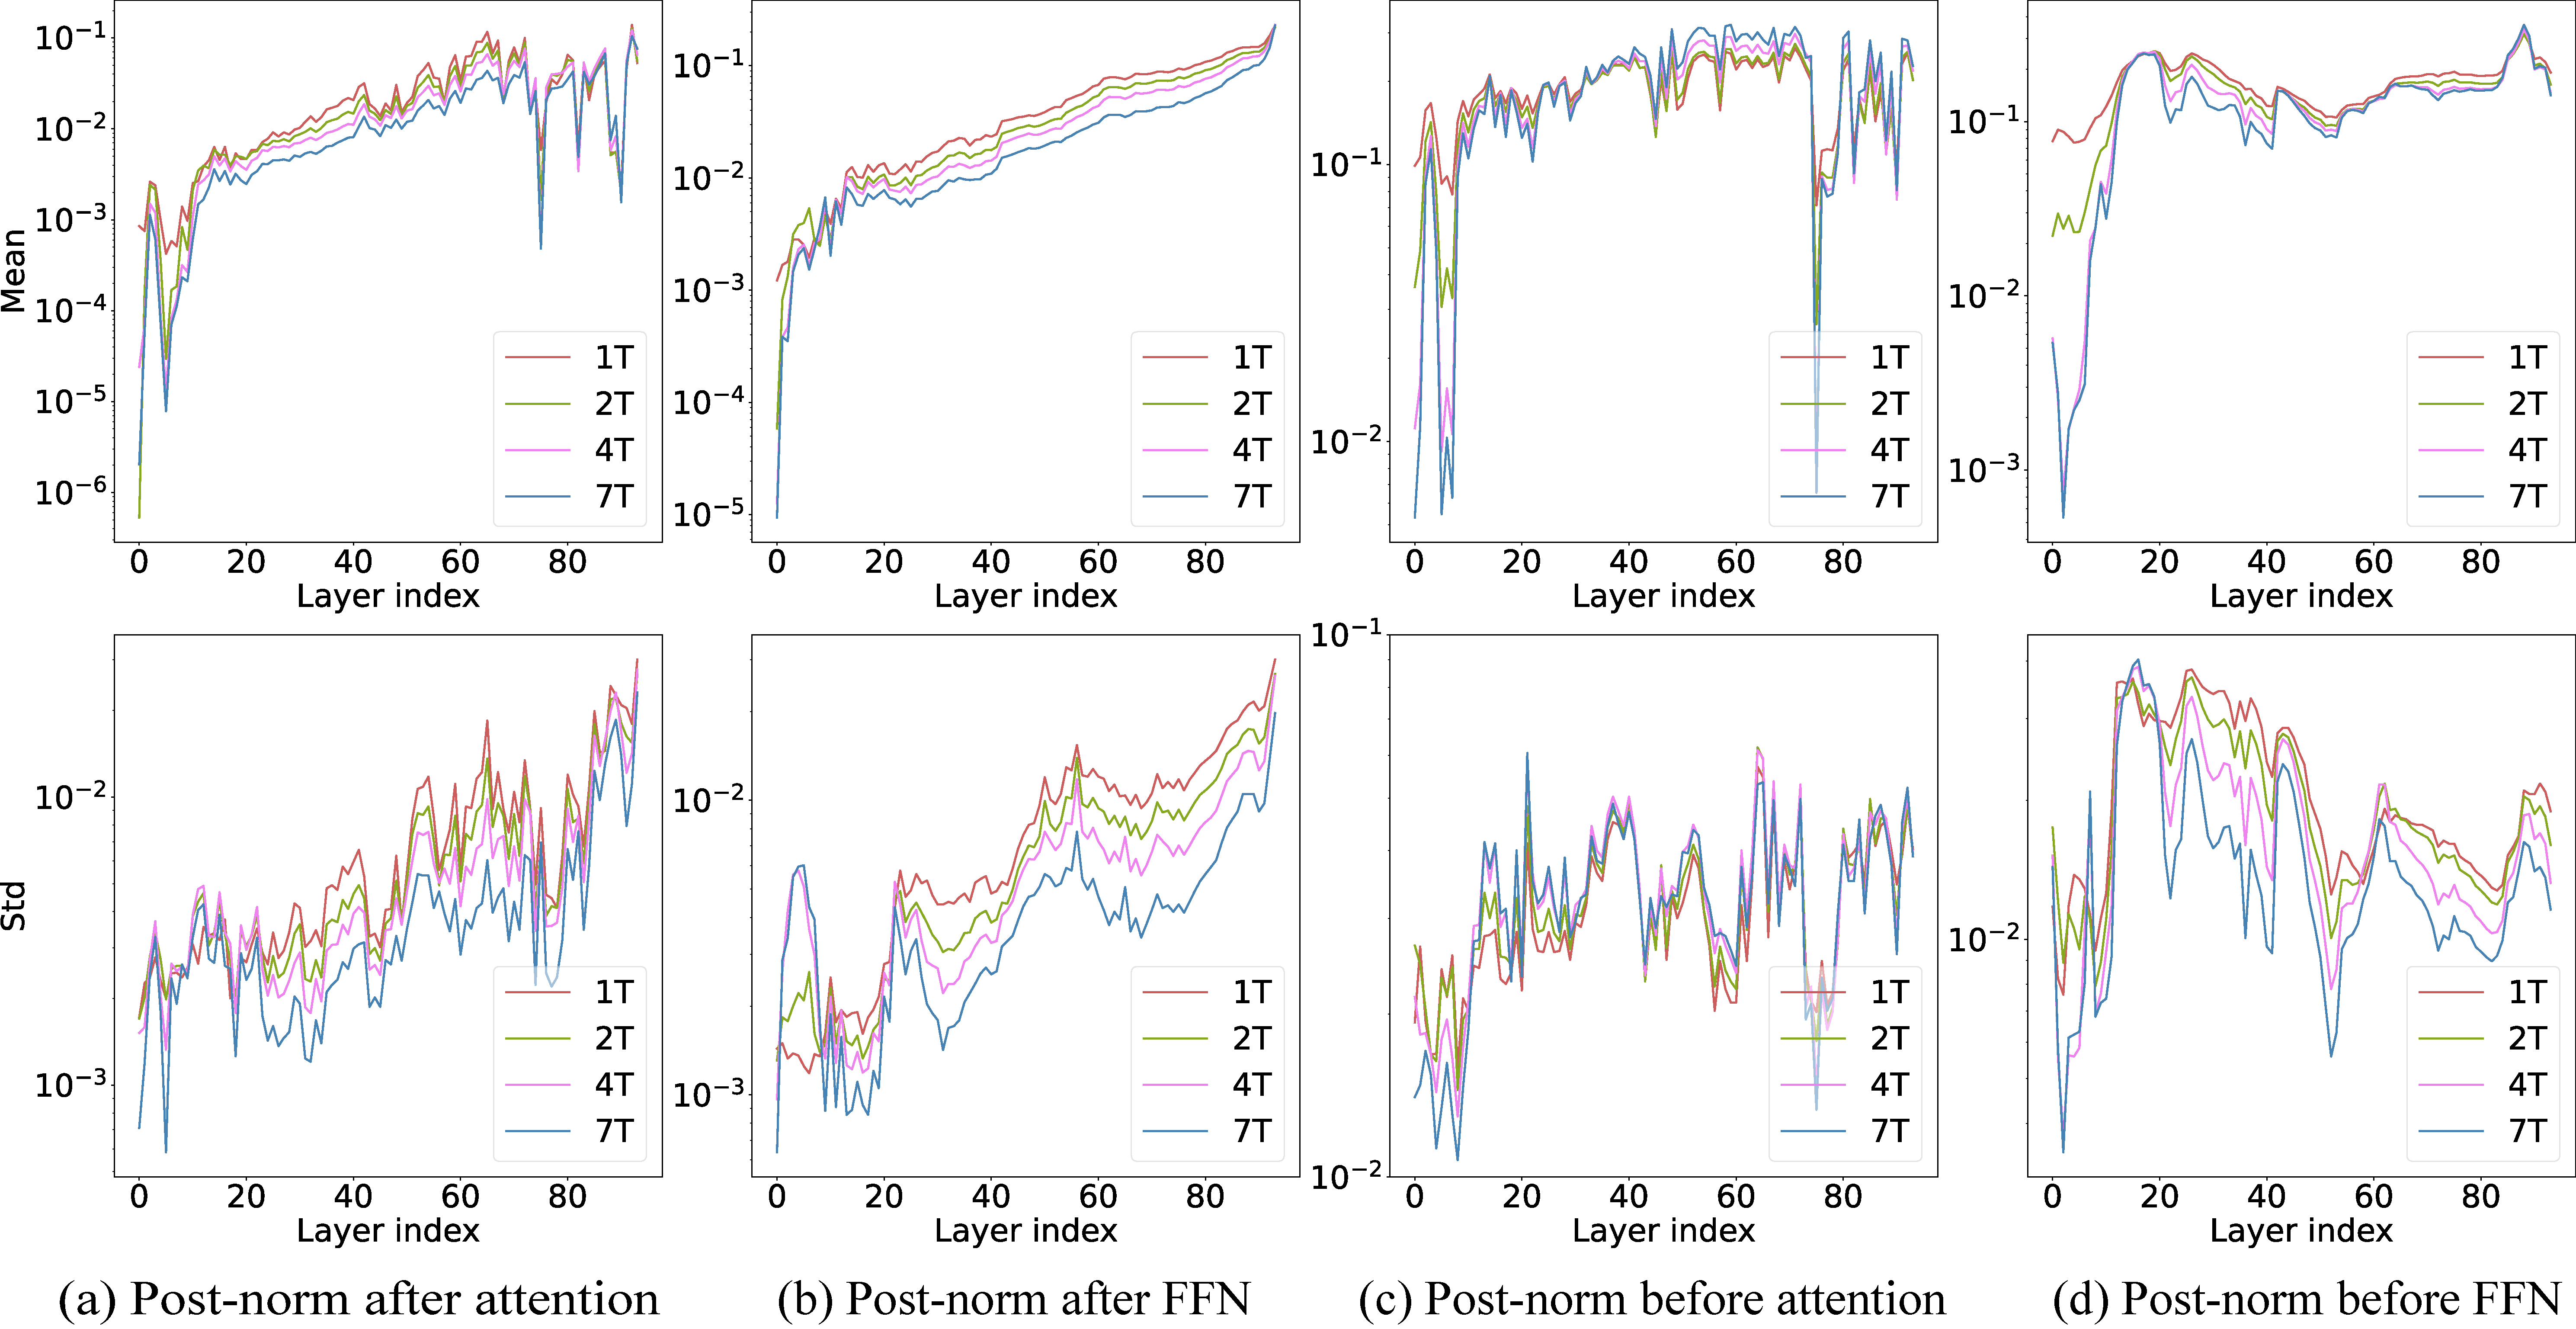
\includegraphics[width=\textwidth]{fig/model_iter_7T_param.pdf}
    \caption{Distribution of sandwich-norm's $\gamma$ parameter. Mean and standard deviation are included. Each line represents different training tokens from 1T, 2T, 4T to 7T. There is a clear layer-wise pattern of the two post-norms: the mean and std value of $\gamma$ increase with depth. Larger post-norm $\gamma$ indicates deeper layers emphasize more on transformer outputs instead of residual connections.}
    \label{fig:gamma_analysis}
\end{figure}
